\documentclass[final, pt]{beamer}

\usepackage[size=a1,orientation=landscape, scale=1.3]{beamerposter}

\usepackage{adjustbox}
\usepackage{caption}
\usepackage{color}
\usepackage{enumitem}
\usepackage{filecontents}
\usepackage{graphicx}
\usepackage{lipsum}
\usepackage{multirow}
\usepackage{pgfmath}
\usepackage{pgfplots}
\usepackage{pgfplotstable}
\usepackage{ragged2e}
\usepackage{soul}
\usepackage{subcaption}
\usepackage{tikz}
\usepackage{transparent}

\usetikzlibrary{arrows.meta}
\usetikzlibrary{calc}
\usetikzlibrary{shadings}

% Define the theme
\usetheme{metropolis}

% Colours
\definecolor{uiored}{HTML}{DD0000}
\definecolor{uiogrey}{HTML}{B2B3B7}
\definecolor{uioblack}{HTML}{000000}
\definecolor{uiowhite}{HTML}{FFFFFF}

% Define the colors
\definecolor{background}{HTML}{FAFAFA}
\setbeamercolor{block title}{bg=background,fg=red}
\setbeamercolor{block body}{bg=background,fg=black}
\setbeamercolor{title}{bg=uiored,fg=uiowhite}
\setbeamercolor{authors}{bg=uioblack,fg=uiowhite}

\setbeamertemplate{page number}{}
\setlength{\paperwidth}{\textwidth}
\setbeamersize{text margin left=0pt, text margin right=0pt}

\def\verticalspace{0.61cm}

\captionsetup[figure]{labelformat=empty}

\definecolor{ADHD}{HTML}{FF0028}
\definecolor{ANX}{HTML}{FF6E00}
\definecolor{ASD}{HTML}{F8FF00}
\definecolor{BIP}{HTML}{5BFF00}
\definecolor{DEM}{HTML}{00FF3B}
\definecolor{MCI}{HTML}{00FFD7}
\definecolor{MDD}{HTML}{008FFF}
\definecolor{MS}{HTML}{0E00FF}
\definecolor{PARK}{HTML}{A600FF}
\definecolor{SCZ}{HTML}{FF00BF}
\definecolor{HC}{HTML}{7F7F7F}

\pgfdeclarelayer{background}
\pgfdeclarelayer{foreground}
\pgfsetlayers{background,main,foreground}

\begin{document}
    \newcommand{\convside}[6]{
        \node[
            fill=#5,
            inner sep=0pt,
            outer sep=0pt,
            minimum width=#3,
            minimum height=#4,
            draw=black
        ] (#6) at (#1, #2) {};
    }

    \newcommand{\convtop}[4]{
        \draw[fill=#4] #1 --
        ($ #1 + (#3, #3) $) --
        ($ #1 + (#3+#2, #3) $) --
        ($ #1 + (#2, 0) $);
    }

    \newcommand{\convfront}[3]{
        \draw[black, fill=#3] #1 --
                            ($ #1 + (1*#2, 1*#2) $) --
                            ($ #1 + (1*#2, 1*#2 - 2*#2) $) --
                            ($ #1 + (0, -2*#2) $);
    }


    \newcommand{\convchannel}[5]{
        \def\huemin{20}
        \def\huemax{80}
        \pgfmathsetmacro{\iterations}{#5-1}
        \foreach \i in {0,...,\iterations} {
            \pgfmathsetmacro{\hue}{int(random(\huemin, \huemax))}
            \convside{#1}{#2+\i*-0.75}{#3}{#4/#5}{black!\hue}{n\i0}
            \convtop{($ (n00.north west) + (0.5*\i*#4/#5, 0.5*\i*#4/#5) $)}{#3}{0.5*#4/#5}{black!\hue}

            \foreach \j in {0,...,\iterations} {
                \pgfmathsetmacro{\innerhue}{int(random(\huemin, \huemax))}
                \ifnum\j=0
                    \pgfmathsetmacro{\innerhue}{\hue}
                \fi
                \convfront{($ (n00.north east) + (0.5*\j*#4/#5, 0.5*\j*#4/#5 - \i*#4/#5) $)}{0.5*#4/#5}{black!\innerhue}
            }
        }
    }

    \newcommand{\convlayer}[6]{
        \pgfmathsetmacro{\iterations}{#6-1}
        \foreach \i in {0,...,\iterations}{
            \pgfmathsetmacro{\x}{#1 + \i * 0.33}
            \convchannel{\x}{#2}{#3}{#4}{#5}
        }
    }

    \newcommand{\cnnarrow}[2]{
        \draw[-stealth, line width=5pt, opacity=0.5] #1 -- #2;
    }

    \newcommand{\cnn}[2]{
        \convlayer{#1}{#2-0.25}{0.33cm}{4.5cm}{6}{3}
        \cnnarrow{(#1 + 1.95, #2 - 1)}{(#1+5.5, #2 - 1)}
        \convlayer{#1 + 5}{#2-0.625}{0.33cm}{3cm}{4}{5}
        \cnnarrow{(#1 + 7.225, #2 - 1)}{(#1+10, #2 - 1)}
        \convlayer{#1 + 9.6}{#2-1}{0.33cm}{1.5cm}{2}{7}
        \cnnarrow{(#1 + 12.125, #2 - 1)}{(#1+14, #2 - 1)}
        \draw[thick, dashed] (#1 - 0.5, #2 + 2.7) --
                            (#1 + 12.9, #2 + 2.7) --
                            (#1 + 12.9, #2 - 4.7) --
                            (#1 - 0.5, #2 - 4.7) -- cycle;
        \node[anchor=south, text depth=0] at (#1 + 6.2, #2 + 2.75) {
            \textbf{\large{Convolutional neural network}}
        };
    }

    \newcommand{\lrpchannel}[5]{
        \def\huemin{0}
        \def\huemax{100}
        \pgfmathsetmacro{\iterations}{#5-1}
        \foreach \i in {0,...,\iterations} {
            \pgfmathsetmacro{\hue}{int(random(\huemin, \huemax))}
            \convside{#1}{#2+\i*-0.75}{#3}{#4/#5}{red!\hue!black}{n\i0}
            \convtop{($ (n00.north west) + (0.5*\i*#4/#5, 0.5*\i*#4/#5) $)}{#3}{0.5*#4/#5}{red!\hue!black}

            \foreach \j in {0,...,\iterations} {
                \pgfmathsetmacro{\innerhue}{int(random(\huemin, \huemax))}
                \ifnum\j=0
                    \pgfmathsetmacro{\innerhue}{\hue}
                \fi
                \convfront{($ (n00.north east) + (0.5*\j*#4/#5, 0.5*\j*#4/#5 - \i*#4/#5) $)}{0.5*#4/#5}{red!\innerhue!black}
            }
        }
    }

    \newcommand{\lrplayer}[6]{
        \pgfmathsetmacro{\iterations}{#6-1}
        \foreach \i in {0,...,\iterations}{
            \pgfmathsetmacro{\x}{#1 + \i * 0.33}
            \lrpchannel{\x}{#2}{#3}{#4}{#5}
        }
    }

    \newcommand{\lrp}[2]{
        \cnnarrow{(#1 - 2.1, #2 - 1)}{(#1+0.5, #2 - 1)}
        \lrplayer{#1}{#2-1}{0.33cm}{1.5cm}{2}{7}
        \cnnarrow{(#1 + 2.525, #2 - 1)}{(#1+5.5, #2 - 1)}
        \lrplayer{#1 + 4.3}{#2-0.625}{0.33cm}{3cm}{4}{5}
        \cnnarrow{(#1 + 6.525, #2 - 1)}{(#1+10, #2 - 1)}
        \lrplayer{#1 + 9}{#2 - 0.25}{0.33cm}{4.5cm}{6}{3}

        \draw[thick, dashed] (#1 - 0.5, #2 + 2.7) --
                            (#1 + 12.4, #2 + 2.7) --
                            (#1 + 12.4, #2 - 4.7) --
                            (#1 - 0.5, #2 - 4.7) -- cycle;
        \node[anchor=south, text depth=0] at (#1 + 5.95, #2 + 2.75) {
            \textbf{\large{Layerwise relevance propagation}}
        };
    }

    \newcommand{\analysisarrow}[2]{
        \draw[-stealth, line width=15pt] #1 -- #2;
    }

    \newcommand{\auctrace}[4]{
        \addplot[
            only marks,
            mark size=10pt,
            mark options={
                fill=#4,
                draw=none,
                opacity=0.5
            }
        ] table [
            col sep=comma,
            x expr=#2,
            y=#3
        ] {data/clinical_predictions/#1/aucs.csv};
    }

    \newcommand{\meantrace}[2]{
        \addplot[black, thick, dashed] coordinates {
            (#1-0.2, #2)
            (#1+0.2, #2)
        };
    }

    \newcommand{\differentiationplot}[3]{
        \begin{tikzpicture}
            \begin{axis}[
                width=20cm,
                height=8cm,
                xmin=0,
                xmax=9,
                ymin=0,
                ymax=1,
                ytick style={draw=none},
                ytick={0, 0.25, 0.5, 0.75, 1},
                yticklabels=#2,
                ylabel=#3,
                xtick={0.5, 1.5, 2.5, 3.5, 4.5, 5.5, 6.5, 7.5, 8.5},
                xticklabels={ADHD, ANX, ASD, BIP, DEM, MCI, MDD, MS, SCZ},
                xtick pos=bottom,
                axis line style ={black},
                clip=false
            ]
                \addplot[gray] coordinates {
                    (0, 0.75)
                    (9, 0.75)
                };
                \addplot[black] coordinates {
                    (0, 0.5)
                    (9, 0.5)
                };
                \addplot[gray] coordinates {
                    (0, 0.25)
                    (9, 0.25)
                };
                \ifnum#1=1
                    \auctrace{ADHD}{0.5}{delta}{gray}
                    \auctrace{ANX}{1.5}{delta}{gray}
                    \auctrace{ASD}{2.5}{delta}{gray}
                    \auctrace{BIP}{3.5}{delta}{gray}
                    \auctrace{DEM}{4.5}{delta}{DEM}
                    \auctrace{MCI}{5.5}{delta}{MCI}
                    \auctrace{MDD}{6.5}{delta}{gray}
                    \auctrace{MS}{7.5}{delta}{MS}
                    \auctrace{SCZ}{8.5}{delta}{SCZ}

                    \node[
                        circle,
                        fill=gray!60,
                        draw=black!60,
                        inner sep=0.24cm
                    ] (insigmarker) at (axis cs: 9.35, 0.19) {};
                    \node[anchor=west] at (insigmarker.east) {p>0.05};
                    \node[
                        circle,
                        draw=black!60,
                        inner sep=0.24cm,
                        anchor=north,
                        upper left=DEM,
                        upper right=MCI,
                        lower left=MS,
                        lower right=SCZ
                    ] (sigmarker) at ($ (insigmarker.south) + (0, -2) $) {};
                    \node[anchor=west] at (sigmarker.east) {p<0.05};
                \fi
                \ifnum#1=2
                    \auctrace{ADHD}{0.5}{maps}{gray}
                    \auctrace{ANX}{1.5}{maps}{gray}
                    \auctrace{ASD}{2.5}{maps}{gray}
                    \auctrace{BIP}{3.5}{maps}{ADHD}
                    \auctrace{DEM}{4.5}{maps}{DEM}
                    \auctrace{MCI}{5.5}{maps}{MCI}
                    \auctrace{MDD}{6.5}{maps}{gray}
                    \auctrace{MS}{7.5}{maps}{MS}
                    \auctrace{SCZ}{8.5}{maps}{SCZ}
                \fi
            \end{axis}
        \end{tikzpicture}
    }

    \newsavebox{\badifferentiation}
    \sbox{\badifferentiation}{%
        \differentiationplot{1}{{0, 0.25, 0.5, 0.75, 1.0}}{\textbf{\Large{AUC}}}
    }

    \newsavebox{\mapdifferentiation}
    \sbox{\mapdifferentiation}{%
        \differentiationplot{2}{\empty}{\empty}
    }

    \newsavebox{\performance}
    \sbox{\performance}{%
        \begin{tikzpicture}
            \begin{axis}[
                height=10cm,
                width=10cm,
                xmin=0,
                xmax=100,
                ymin=0,
                ymax=100,
                xlabel={Predicted brain age},
                ylabel={Chronological brain age}
            ]
                \addplot[black] coordinates {(0, 0) (100, 100)};
                \addplot[
                    only marks,
                    MDD,
                    mark size=5pt,
                    mark options={
                        line width=1pt,
                        draw=black,
                        opacity=0.5
                    }
                ] table [
                    col sep=comma,
                    x=prediction,
                    y=age
                ] {data/brain_age_predictions.csv};
                \node[anchor=south east] at (axis cs: 100, 0) {\textbf{MAE=4.51}};

            \end{axis}
        \end{tikzpicture}
    }

    \newsavebox{\diagnoses}
    \sbox{\diagnoses}{%
        \begin{tikzpicture}
            \def\mriwidth{5cm}
            \node[minimum height=\mriwidth, fill=black, inner sep=0pt] (ADHD)at (0, 0) {
                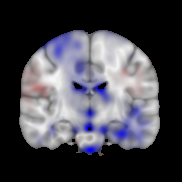
\includegraphics[width=\mriwidth]{data/averages/ADHD/diff.png}
            };
            \node[minimum height=\mriwidth, fill=black, inner sep=0pt] (ANX) at (\mriwidth, 0) {
                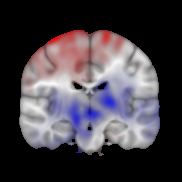
\includegraphics[width=\mriwidth]{data/averages/ANX/diff.png}
            };
            \node[minimum height=\mriwidth, fill=black, inner sep=0pt] (ASD) at (\mriwidth * 2, 0) {
                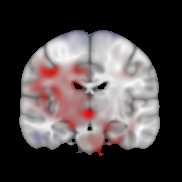
\includegraphics[width=\mriwidth]{data/averages/ASD/diff.png}
            };

            \node[minimum height=\mriwidth, fill=black, inner sep=0pt] (BIP) at (0, -\mriwidth) {
                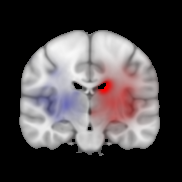
\includegraphics[width=\mriwidth]{data/averages/BIP/diff.png}
            };
            \node[minimum height=\mriwidth, fill=black, inner sep=0pt] (DEM) at (\mriwidth, -\mriwidth) {
                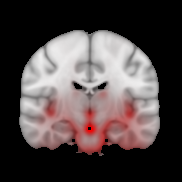
\includegraphics[width=\mriwidth]{data/averages/DEM/diff.png}
            };
            \node[minimum height=\mriwidth, fill=black, inner sep=0pt] (MCI) at (\mriwidth * 2, -\mriwidth) {
                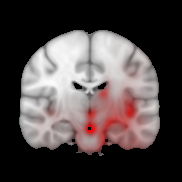
\includegraphics[width=\mriwidth]{data/averages/MCI/diff.png}
            };

            \node[minimum height=\mriwidth, fill=black, inner sep=0pt] (MDD) at (0, -2 * \mriwidth) {
                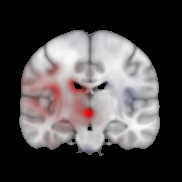
\includegraphics[width=\mriwidth]{data/averages/MDD/diff.png}
            };
            \node[minimum height=\mriwidth, fill=black, inner sep=0pt] (MS) at (\mriwidth, -2 * \mriwidth) {
                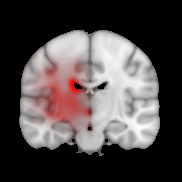
\includegraphics[width=\mriwidth]{data/averages/MS/diff.png}
            };
            \node[minimum height=\mriwidth, fill=black, inner sep=0pt] (SCZ) at (\mriwidth * 2, -2 * \mriwidth) {
                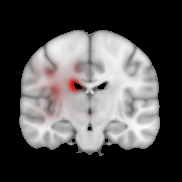
\includegraphics[width=\mriwidth]{data/averages/SCZ/diff.png}
            };

            \def\textsep{0.6}
            \foreach \diagnosis in {ADHD, ANX, ASD, BIP, DEM, MCI, MDD, MS, SCZ} {
                \node[minimum width=\mriwidth, fill=black, anchor=south, text=white] at ($ (\diagnosis.north) - (0, \textsep) $) {\diagnosis};
            }
        \end{tikzpicture}
    }

    \newsavebox{\overview}
    \sbox{\overview}{%
        \def\nodesize{1cm}
        \def\predictfill{blue}
        \begin{tikzpicture}
            \node[yslant=1] (input) at (1.1, -7.5) {
                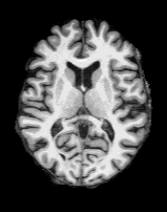
\includegraphics[height=4cm]{data/mri.png}
            };
            \node[
                anchor=south west,
                align=center,
                font=\normalfont\linespread{0.8}\selectfont
            ] at ($ (input.east) - (0, 1.8) $) {
                T1-weighted\\
                structural MRI
            };
            \node[align=center,font=\large\linespread{0.8}\selectfont, text depth=0] (prediction) at (27.5, -7.5) {
                Brain age gap
            };

            \cnnarrow{(1.1, -7.5)}{(10.5, -7.5)}
            \cnn{10}{-6.5}

            \lrp{33}{-6.5}
            \cnnarrow{(42.95, -7.5)}{(53, -7.5)}

            \node[yslant=1] (map) at (53, -7.5) {
                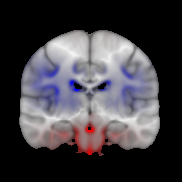
\includegraphics[height=4cm]{data/heatmap.png}
            };
            \node[
                anchor=south east,
                align=center,
                font=\normalfont\linespread{0.8}\selectfont
            ] at ($ (map.west) + (-0.5, 1.8) $) {
                Explanatory\\
                heatmaps
            };

            \node[anchor=north] (babox) at ($ (prediction) - (1.55, 5.5) $) {
                \usebox{\badifferentiation}
            };
            \node[anchor=south] at ($ (babox.north) + (1.15, -1) $) {
                \textbf{\large{Case/control predictions}}
            };
            \node[anchor=north] (mapbox) at ($ (map) - (0.42, 5.77) $) {
                \usebox{\mapdifferentiation}
            };
            \node[anchor=south] at ($ (mapbox.north) + (0, -0.73) $) {
                \textbf{\large{Case/control predictions}}
            };
            \node[anchor=south] (correlations) at ($ (prediction.north) + (-1, 3.7) $) {
                \usebox{\performance}
            };
            \node[anchor=south] at ($ (correlations.north) + (1,-0.8) $) {
                \textbf{\large{Model evaluation}}
            };
            \node[anchor=west] (diagnoses) at (63, -7.5) {
                \usebox{\diagnoses}
            };
            \node[anchor=south] at ($ (diagnoses.north) + (0, -0.5) $) {
                \textbf{\large{Average heatmaps}}
            };

            \analysisarrow{($ (prediction.south) - (0, 0.5) $)}{($ (babox.north) + (1.55, 0.4) $)}
            \analysisarrow{($ (prediction.north) + (0, 0.5) $)}{($ (correlations.south) + (1, 0.2) $)}
            \analysisarrow{($ (map.south) - (0, 0.5) $)}{($ (mapbox.north) + (0.42, 0.6) $)}
            \analysisarrow{($ (map.east) + (1, -1.92) $)}{($ (diagnoses.west) + (0, 0) $)}

        \end{tikzpicture}
    }


    \def\authorfont{\large}
    \def\sectionwidth{0.235\textwidth}

    \newcommand{\postersection}[3]{
        \begin{minipage}[t][#2][t]{\textwidth}
            \LARGE{\textcolor{uiored}{#1}}\\[-0.5cm]
            \rule{\textwidth}{1pt}\\[0.3cm]
            \fontsize{24}{23}\selectfont
            #3
        \end{minipage}
    }

    % Start the poster
    \begin{frame}[t]
        \thispagestyle{empty}

    % Title and author block
        \begin{beamercolorbox}[sep=0em,wd=\textwidth]{title}
            \begin{columns}
                \begin{column}{0.2\textwidth}
                \end{column}
                \begin{column}{0.6\textwidth}
                    \centering\\[2.5cm]
                    \fontsize{60}{70}{
                        \textbf{Increasing the sensitivity of brain age modelling}\\[0.5cm]
                        \textbf{with explainable artificial intelligence}
                    }
                    \vspace{2.5cm}
                \end{column}
                \begin{column}{0.2\textwidth}
                \end{column}
            \end{columns}
        \end{beamercolorbox}

        \begin{beamercolorbox}[sep=0em, wd=\textwidth]{authors}
            \def\authorwidth{.16\textwidth}
            \begin{columns}[T]
                \begin{column}{\authorwidth}
                    \centering
                    \vspace{-0.3cm}
                    \authorfont{Esten H. Leonardsen}\\
                    \authorfont{University of Oslo}\\
                    \vspace{0.3cm}
                \end{column}
                \begin{column}{\authorwidth}
                    \centering
                    \vspace{-0.25cm}
                    \authorfont{Yunpeng Wang}\\
                    \authorfont{University of Oslo}
                \end{column}
                \begin{column}{\authorwidth}
                    \centering
                    \vspace{-0.3cm}
                    \authorfont{Lars T. Westlye}\\
                    \authorfont{University of Oslo}
                \end{column}
                \begin{column}{\authorwidth}
                    \centering
                    \vspace{-0.3cm}
                    \authorfont{Thomas Wolfers}\\
                    \authorfont{University of Tübingen}
                \end{column}
            \end{columns}
        \end{beamercolorbox}

        \vspace{0.4cm}
        \begin{center}
            \usebox{\overview}
        \end{center}
        \vspace{0.4cm}

        \begin{columns}
            \begin{column}{\sectionwidth}
                \postersection{Introduction}{25cm}{
                    The brain age gap (BAG), a neuroimaging-derived measure encoding the difference between the apparent and chronological age of the brain, has gained popularity as a biomarker of generalized brain health. A multitude of studies have revealed older-appearing brains in patients with various conditions\textsuperscript{1}. However, while a discrepancy can be evident at the group-level, the abstract and summarizing nature of BAG limits its utility for precise, individualized clinical decision-making. Explainable artificial intelligence (XAI) can unveil brain regions causing deviations in BAG in the individual patient, providing a data modality that is plausibly more useful than the singular measure\textsuperscript{2}.
                }
            \end{column}
            \begin{column}{\sectionwidth}
                \postersection{Methods}{25cm}{
                    We trained a convolutional neural network to predict BAG using 80,007 structural magnetic resonance images from 67,881 participants. On top of the model we implemented layer-wise relevance propagation to procure heatmaps highlighting regions underlying a deviating BAG in individual participants. Finally, we investigated whether these heatmaps could support clinical decision-making across nine conditions: Attention-deficit/hyperactivity disorder (ADHD), anxiety disorders (ANX), autism spectrum disorder (ASD), bipolar disorder (BIP), dementia (DEM), mild cognitive impairment (MCI), major depressive disorder (MDD), multiple sclerosis (MS) and schizophrenia (SCZ).
                }
            \end{column}
            \begin{column}{\sectionwidth}
                \postersection{Results}{25cm}{
                    Our model achieved satisfactory predictive performance in a held-out dataset (mean absolute error=4.51) from unknown scanners. Singular BAGs from our model allowed us to meaningfully discriminate patients from controls (mean area under the receiver operating curve (AUC)>0.5 in a nested 10-fold cross-validation, p<0.05) for four out of nine diagnoses (DEM, MCI, MS, SCZ). The heatmaps yielded significantly improved predictions (mean AUC\textsubscript{map}>mean AUC\textsubscript{BAG}, p<0.05) for five out of nine diagnoses (BIP, DEM, MCI, MS, SCZ). Visual inspection of average heatmaps per patient cohort revealed that the highlighted regions varied notably between conditions.
                }
            \end{column}
            \begin{column}{\sectionwidth}
                \begin{minipage}[t][25cm][t]{\textwidth}
                    \postersection{Conclusion}{6.53cm}{
                        Enhancing brain age models with XAI techniques  introduces a new, derived, data modality that is more sensitive towards subtle aberrations in neuroimaging data than a singular brain age prediction.
                    }
                    \postersection{References}{10cm}{
                        1. Franke, K. \& Gaser, C. Ten Years of BrainAGE as a Neuroimaging Biomarker of Brain Aging: What Insights Have We Gained? \textit{Frontiers in Neurology}, 2019\\
                        2. Martin S.A. et al. Interpretable machine learning for dementia: A systematic review. \textit{Alzheimer's Dementia}, 2023
                    }
                \end{minipage}
            \end{column}
        \end{columns}
    \end{frame}
\end{document}

% TODO:
% Better title
% UiO-logo
% QR-code
% Mean AUCs in plot
% New MRI/heatmap
% Better LRP colouring
